\chapter{Unfolding procedure of fake muon control sample}
\label{appx:unfold-tech}

The notation that we use in the main text and throughout this appendix is as follows:

\begin{itemize}
\item Hats as that in $\hat{t}$ refer to species tagged as a track of species $t$ based
  on the cuts listed in \cref{tab:selection-for-tagged-species} or the \muon PID.
\item Apostrophes as that in $t'$ are used simply to indicate that the track species may or may not
  be the same that in $t$.
\item Subscripts such as $t_\text{fake}$ indicate which selection the event satisfies.
\item Yields denoted with the letter $n$ refer to the number of events in the \pidcalib (or MC) samples, while
  yields with tilde ($\tilde{n}$) refer the number of events in our $D^{(*)}\mu$ or $D^{(*)}h$ samples.
\end{itemize}

The various samples considered in this procedure are described below and shown
schematically in \cref{fig:relation-unfolding-sets}:

\begin{itemize}
\item $t_\text{PIDCalib}$: The \pidcalib sample (or MC in the case of ghosts) with minimal cuts
  that is considered to be pure in the track species $t$.
\item $t_\text{acc}$: The subset of $t_\text{PIDCalib}$ that satisfies all \muon
cuts other than PID (ie, track in \muon acceptance).
\item $t_\text{fake}$: The subset of $t_{acc}$ that \emph{fails} \muon PID and thus falls
  into the fake \muon sample.
\item $\hat{\mu}_\text{sig}$: The subset of $t_{acc}$ that \emph{passes} \muon PID
  and thus falls into the signal sample.
\item $\hat{t}'_\text{fake}$: The subset of $t_\text{fake}$ that passes the $\hat{t}'$ tagging requirements
  from \cref{tab:selection-for-tagged-species}.
\end{itemize}

\begin{figure}[ht]
    \centering
    \resizebox{0.9\columnwidth}{!}{
        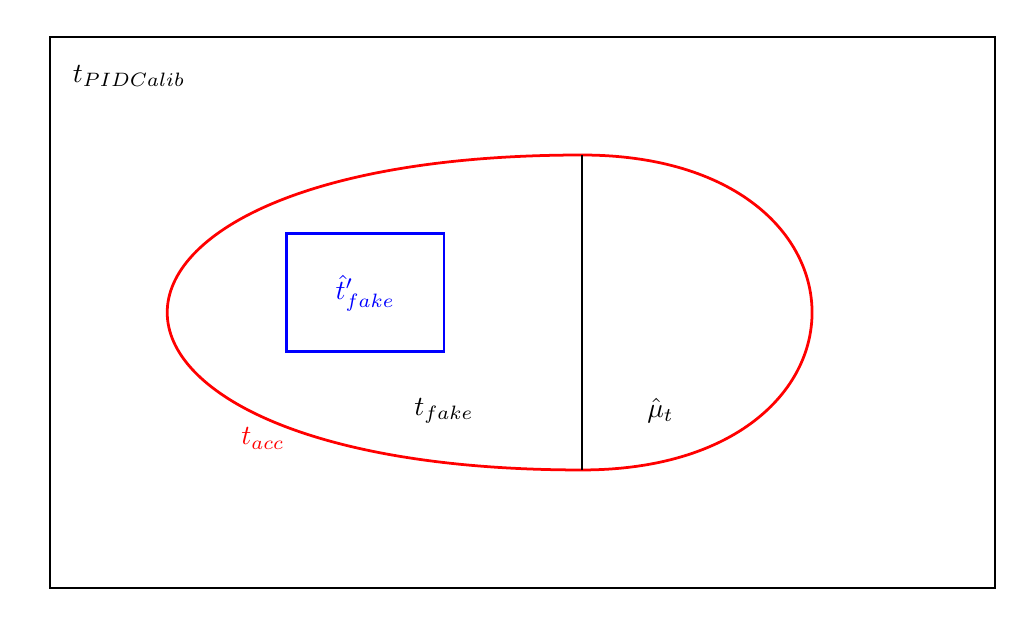
\begin{tikzpicture}
    \pgfdeclarelayer{nodelayer}
    \pgfdeclarelayer{edgelayer}
    \pgfsetlayers{nodelayer,edgelayer}

	\begin{pgfonlayer}{nodelayer}
		\node (0) at (-6, -3.5) {};
		\node (1) at (6, -3.5) {};
		\node (2) at (-6, 3.5) {};
		\node (3) at (6, 3.5) {};
		\node (6) at (-5, 3) {$t_\text{PIDCalib}$};
		\node (7) at (-6, 3) {};
		\node (8) at (-6, -3) {};
		\node (9) at (6, -3) {};
		\node (10) at (6, 3) {};
        \node[red] (11) at (-3.3, -1.6) {$t_\text{acc}$};
		\node (14) at (0.75, -2) {};
		\node (15) at (0.75, 2) {};
		\node (17) at (-1, -1.25) {$t_\text{fake}$};
		\node (18) at (1.75, -1.25) {$\hat{\mu}_t$};
		\node (19) at (-3, 1) {};
		\node (20) at (-3, -0.5) {};
		\node (21) at (-1, -0.5) {};
		\node (22) at (-1, 1) {};
		\node (23) at (-2, 0.25) {};
        \node[blue] (24) at (-2, 0.25) {$\hat{t}'_\text{fake}$};
	\end{pgfonlayer}
	\begin{pgfonlayer}{edgelayer}
        \draw[line width=0.3mm] (1.center)
			 to (0.center)
			 to (2.center)
			 to (3.center)
			 to cycle;
        \draw[red, line width=0.35mm] (15.center)
			 to [in=180, out=180, looseness=4.50] (14.center)
			 to [in=0, out=0, looseness=2.50] cycle;
        \draw[line width=0.3mm] (15.center)
			 to (14.center);
        \draw[blue, line width=0.35mm] (19.center)
			 to (22.center)
			 to (21.center)
			 to (20.center)
			 to cycle;
	\end{pgfonlayer}
\end{tikzpicture}

    }
    \caption{Relations between $t$-specie-enriched samples used in unfolding.}
    \label{fig:relation-unfolding-sets}
\end{figure}


We now describe step 2 and 3 in the main text with more detail.

\paragraph{Step 2} The probability of a true $t$ to be classified as $\hat{t}'$ can
be computed as:

\begin{equation}
    \misEff[t]{\hat{t}'} = \frac{n_{\hat{t}'}}{n_{t}}
\end{equation}

where $n$ denote yields, and subscripts denote sample following the nomenclature
explained above. Note that all efficiencies are binned in $p_B$, $\eta_B$, and
nTracks with a consistent binning scheme.


\paragraph{Step 3} In a particular bin, the measured
yields $\tilde{n}_{\hat{t}'}$, the true yields $\tilde{n}_{t}$, and the response matrix $M$
have the following relation (all yields and efficiencies are in the fake \muon sample but
the \emph{fake} subscript is dropped for readability):

\begin{equation}
    \begin{pmatrix*}[l]
        \tilde{n}_{\hat{\pi}} \\
        \tilde{n}_{\hat{K}}   \\
        \tilde{n}_{\hat{p}}   \\
        \tilde{n}_{\hat{e}}   \\
        \tilde{n}_{\hat{g}}   \\
    \end{pmatrix*}
    =
    \begin{pmatrix*}[l]
        \misEff[\pi]{\hat{\pi}} & \misEff[K]{\hat{\pi}} & \misEff[p]{\hat{\pi}} & \misEff[e]{\hat{\pi}} & \misEff[g]{\hat{\pi}} \\
        \misEff[\pi]{\hat{K}}   & \misEff[K]{\hat{K}}   & \misEff[p]{\hat{K}}   & \misEff[e]{\hat{K}}   & \misEff[g]{\hat{K}}   \\
        \misEff[\pi]{\hat{p}}   & \misEff[K]{\hat{p}}   & \misEff[p]{\hat{p}}   & \misEff[e]{\hat{p}}   & \misEff[g]{\hat{p}}   \\
        \misEff[\pi]{\hat{e}}   & \misEff[K]{\hat{e}}   & \misEff[p]{\hat{e}}   & \misEff[e]{\hat{e}}   & \misEff[g]{\hat{e}}   \\
        \misEff[\pi]{\hat{g}}   & \misEff[K]{\hat{g}}   & \misEff[p]{\hat{g}}   & \misEff[e]{\hat{g}}   & \misEff[g]{\hat{g}}   \\
    \end{pmatrix*}
    \begin{pmatrix*}[l]
        \tilde{n}_{{\pi}} \\
        \tilde{n}_{{K}}   \\
        \tilde{n}_{{p}}   \\
        \tilde{n}_{{e}}   \\
        \tilde{n}_{{g}}   \\
    \end{pmatrix*}
\end{equation}
where $\tilde{n}$ denote yields. The tilde indicates that $t/\hat{t}'$ refer to
the true/tagged species reconstructed from the fake $\mu$ samples,
and the nomenclature introduced in the beginning of the appendix does not apply.

The Bayesian (iterative) unfolding method provided by \RooUnfold\ is used to
obtain the true yields.
Naive matrix inversion cannot be used because it is sensitive to statistical
fluctuations.  % TODO: Should I cite Cowan here?

To find $\misEff[\hat{t}_\text{fake}']{t_\text{fake}}$, recall its definition:

\begin{equation}
    \misEff[\hat{t}_\text{fake}']{t_\text{fake}} \equiv
        \frac{
            \text{Number of $\hat{t}'$ from $t$}
        }{
            \text{Total number of $\hat{t}'$ based on unfolding}
        }
\end{equation}

With the unfolded true yields, we can compute:

\begin{itemize}
    \item Number of $\hat{t}'$ from $t$:
        $\tilde{n}_t \cdot \misEff[t_\text{fake}]{\hat{t}_\text{fake}'}$
    \item Total number of $\hat{t}'$ based on unfolding:
        $\sum_t \tilde{n}_t \cdot \misEff[t_\text{fake}]{\hat{t}_\text{fake}'}$
\end{itemize}

Therefore:

\begin{equation}
    \misEff[\hat{t}_\text{fake}']{t_\text{fake}} =
        \frac{
            \tilde{n}_t \cdot \misEff[t_\text{fake}]{\hat{t}_\text{fake}'}
        }{
            \sum_t \tilde{n}_t \cdot \misEff[t_\text{fake}]{\hat{t}_\text{fake}'}
        }
\end{equation}
